% Options for packages loaded elsewhere
\PassOptionsToPackage{unicode}{hyperref}
\PassOptionsToPackage{hyphens}{url}
%
\documentclass[
]{article}
\usepackage{amsmath,amssymb}
\usepackage{lmodern}
\usepackage{iftex}
\ifPDFTeX
  \usepackage[T1]{fontenc}
  \usepackage[utf8]{inputenc}
  \usepackage{textcomp} % provide euro and other symbols
\else % if luatex or xetex
  \usepackage{unicode-math}
  \defaultfontfeatures{Scale=MatchLowercase}
  \defaultfontfeatures[\rmfamily]{Ligatures=TeX,Scale=1}
\fi
% Use upquote if available, for straight quotes in verbatim environments
\IfFileExists{upquote.sty}{\usepackage{upquote}}{}
\IfFileExists{microtype.sty}{% use microtype if available
  \usepackage[]{microtype}
  \UseMicrotypeSet[protrusion]{basicmath} % disable protrusion for tt fonts
}{}
\makeatletter
\@ifundefined{KOMAClassName}{% if non-KOMA class
  \IfFileExists{parskip.sty}{%
    \usepackage{parskip}
  }{% else
    \setlength{\parindent}{0pt}
    \setlength{\parskip}{6pt plus 2pt minus 1pt}}
}{% if KOMA class
  \KOMAoptions{parskip=half}}
\makeatother
\usepackage{xcolor}
\IfFileExists{xurl.sty}{\usepackage{xurl}}{} % add URL line breaks if available
\IfFileExists{bookmark.sty}{\usepackage{bookmark}}{\usepackage{hyperref}}
\hypersetup{
  pdftitle={Chapter 23},
  pdfauthor={Alan T. Arnholt},
  hidelinks,
  pdfcreator={LaTeX via pandoc}}
\urlstyle{same} % disable monospaced font for URLs
\usepackage[margin=1in]{geometry}
\usepackage{color}
\usepackage{fancyvrb}
\newcommand{\VerbBar}{|}
\newcommand{\VERB}{\Verb[commandchars=\\\{\}]}
\DefineVerbatimEnvironment{Highlighting}{Verbatim}{commandchars=\\\{\}}
% Add ',fontsize=\small' for more characters per line
\usepackage{framed}
\definecolor{shadecolor}{RGB}{248,248,248}
\newenvironment{Shaded}{\begin{snugshade}}{\end{snugshade}}
\newcommand{\AlertTok}[1]{\textcolor[rgb]{0.94,0.16,0.16}{#1}}
\newcommand{\AnnotationTok}[1]{\textcolor[rgb]{0.56,0.35,0.01}{\textbf{\textit{#1}}}}
\newcommand{\AttributeTok}[1]{\textcolor[rgb]{0.77,0.63,0.00}{#1}}
\newcommand{\BaseNTok}[1]{\textcolor[rgb]{0.00,0.00,0.81}{#1}}
\newcommand{\BuiltInTok}[1]{#1}
\newcommand{\CharTok}[1]{\textcolor[rgb]{0.31,0.60,0.02}{#1}}
\newcommand{\CommentTok}[1]{\textcolor[rgb]{0.56,0.35,0.01}{\textit{#1}}}
\newcommand{\CommentVarTok}[1]{\textcolor[rgb]{0.56,0.35,0.01}{\textbf{\textit{#1}}}}
\newcommand{\ConstantTok}[1]{\textcolor[rgb]{0.00,0.00,0.00}{#1}}
\newcommand{\ControlFlowTok}[1]{\textcolor[rgb]{0.13,0.29,0.53}{\textbf{#1}}}
\newcommand{\DataTypeTok}[1]{\textcolor[rgb]{0.13,0.29,0.53}{#1}}
\newcommand{\DecValTok}[1]{\textcolor[rgb]{0.00,0.00,0.81}{#1}}
\newcommand{\DocumentationTok}[1]{\textcolor[rgb]{0.56,0.35,0.01}{\textbf{\textit{#1}}}}
\newcommand{\ErrorTok}[1]{\textcolor[rgb]{0.64,0.00,0.00}{\textbf{#1}}}
\newcommand{\ExtensionTok}[1]{#1}
\newcommand{\FloatTok}[1]{\textcolor[rgb]{0.00,0.00,0.81}{#1}}
\newcommand{\FunctionTok}[1]{\textcolor[rgb]{0.00,0.00,0.00}{#1}}
\newcommand{\ImportTok}[1]{#1}
\newcommand{\InformationTok}[1]{\textcolor[rgb]{0.56,0.35,0.01}{\textbf{\textit{#1}}}}
\newcommand{\KeywordTok}[1]{\textcolor[rgb]{0.13,0.29,0.53}{\textbf{#1}}}
\newcommand{\NormalTok}[1]{#1}
\newcommand{\OperatorTok}[1]{\textcolor[rgb]{0.81,0.36,0.00}{\textbf{#1}}}
\newcommand{\OtherTok}[1]{\textcolor[rgb]{0.56,0.35,0.01}{#1}}
\newcommand{\PreprocessorTok}[1]{\textcolor[rgb]{0.56,0.35,0.01}{\textit{#1}}}
\newcommand{\RegionMarkerTok}[1]{#1}
\newcommand{\SpecialCharTok}[1]{\textcolor[rgb]{0.00,0.00,0.00}{#1}}
\newcommand{\SpecialStringTok}[1]{\textcolor[rgb]{0.31,0.60,0.02}{#1}}
\newcommand{\StringTok}[1]{\textcolor[rgb]{0.31,0.60,0.02}{#1}}
\newcommand{\VariableTok}[1]{\textcolor[rgb]{0.00,0.00,0.00}{#1}}
\newcommand{\VerbatimStringTok}[1]{\textcolor[rgb]{0.31,0.60,0.02}{#1}}
\newcommand{\WarningTok}[1]{\textcolor[rgb]{0.56,0.35,0.01}{\textbf{\textit{#1}}}}
\usepackage{longtable,booktabs,array}
\usepackage{calc} % for calculating minipage widths
% Correct order of tables after \paragraph or \subparagraph
\usepackage{etoolbox}
\makeatletter
\patchcmd\longtable{\par}{\if@noskipsec\mbox{}\fi\par}{}{}
\makeatother
% Allow footnotes in longtable head/foot
\IfFileExists{footnotehyper.sty}{\usepackage{footnotehyper}}{\usepackage{footnote}}
\makesavenoteenv{longtable}
\usepackage{graphicx}
\makeatletter
\def\maxwidth{\ifdim\Gin@nat@width>\linewidth\linewidth\else\Gin@nat@width\fi}
\def\maxheight{\ifdim\Gin@nat@height>\textheight\textheight\else\Gin@nat@height\fi}
\makeatother
% Scale images if necessary, so that they will not overflow the page
% margins by default, and it is still possible to overwrite the defaults
% using explicit options in \includegraphics[width, height, ...]{}
\setkeys{Gin}{width=\maxwidth,height=\maxheight,keepaspectratio}
% Set default figure placement to htbp
\makeatletter
\def\fps@figure{htbp}
\makeatother
\setlength{\emergencystretch}{3em} % prevent overfull lines
\providecommand{\tightlist}{%
  \setlength{\itemsep}{0pt}\setlength{\parskip}{0pt}}
\setcounter{secnumdepth}{5}
\ifLuaTeX
  \usepackage{selnolig}  % disable illegal ligatures
\fi

\title{Chapter 23}
\author{Alan T. Arnholt}
\date{Last compiled: May 10, 2022 at 09:29:20 AM}

\begin{document}
\maketitle

{
\setcounter{tocdepth}{2}
\tableofcontents
}
\hypertarget{inferences-for-regression}{%
\section{Inferences for Regression}\label{inferences-for-regression}}

\begin{Shaded}
\begin{Highlighting}[]
\NormalTok{bodyfat }\OtherTok{\textless{}{-}} \FunctionTok{read.csv}\NormalTok{(}\StringTok{"./DATA/Bodyfat.csv"}\NormalTok{) }\SpecialCharTok{\%\textgreater{}\%} 
  \FunctionTok{clean\_names}\NormalTok{()}
\FunctionTok{head}\NormalTok{(bodyfat)}
\end{Highlighting}
\end{Shaded}

\begin{verbatim}
  density pct_bf age weight height neck chest abdomen    waist   hip thigh knee
1  1.0708   12.3  23 154.25  67.75 36.2  93.1    85.2 33.54331  94.5  59.0 37.3
2  1.0853    6.1  22 173.25  72.25 38.5  93.6    83.0 32.67717  98.7  58.7 37.3
3  1.0414   25.3  22 154.00  66.25 34.0  95.8    87.9 34.60630  99.2  59.6 38.9
4  1.0751   10.4  26 184.75  72.25 37.4 101.8    86.4 34.01575 101.2  60.1 37.3
5  1.0340   28.7  24 184.25  71.25 34.4  97.3   100.0 39.37008 101.9  63.2 42.2
6  1.0502   20.9  24 210.25  74.75 39.0 104.5    94.4 37.16535 107.8  66.0 42.0
  ankle bicep forearm wrist
1  21.9  32.0    27.4  17.1
2  23.4  30.5    28.9  18.2
3  24.0  28.8    25.2  16.6
4  22.8  32.4    29.4  18.2
5  24.0  32.2    27.7  17.7
6  25.6  35.7    30.6  18.8
\end{verbatim}

\begin{Shaded}
\begin{Highlighting}[]
\FunctionTok{ggplot}\NormalTok{(}\AttributeTok{data =}\NormalTok{ bodyfat, }\FunctionTok{aes}\NormalTok{(}\AttributeTok{x =}\NormalTok{ waist, }\AttributeTok{y =}\NormalTok{ pct\_bf)) }\SpecialCharTok{+} 
  \FunctionTok{geom\_point}\NormalTok{(}\AttributeTok{color =} \StringTok{"blue"}\NormalTok{) }\SpecialCharTok{+}
  \FunctionTok{theme\_bw}\NormalTok{() }\SpecialCharTok{+} 
  \FunctionTok{labs}\NormalTok{(}\AttributeTok{x =} \StringTok{"Waist (in.)"}\NormalTok{, }\AttributeTok{y =} \StringTok{"\% Body Fat"}\NormalTok{)}
\end{Highlighting}
\end{Shaded}

\begin{figure}

{\centering 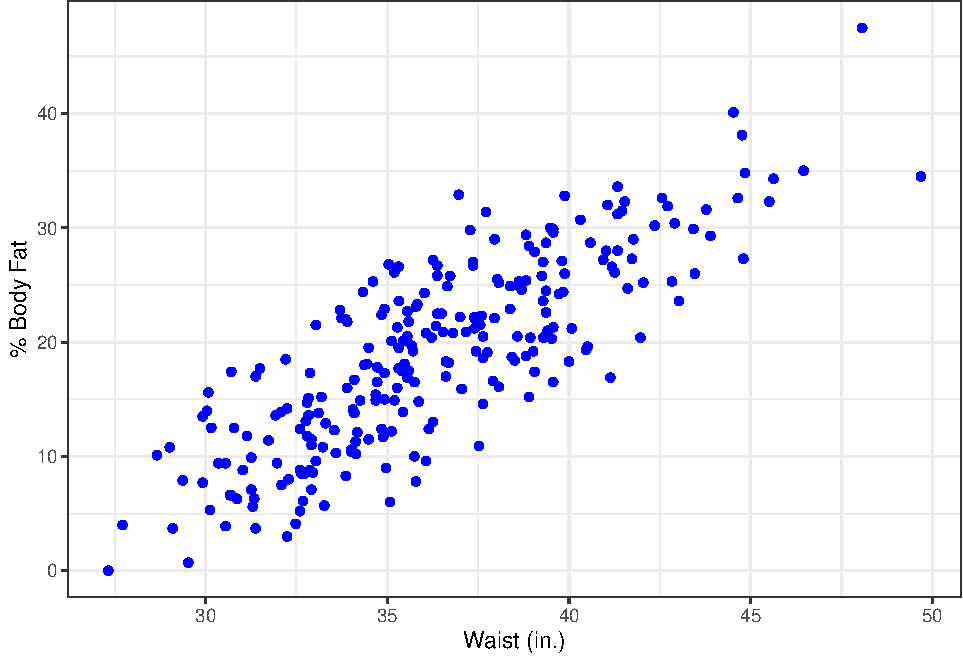
\includegraphics{CHAP23_files/figure-latex/fig231-1} 

}

\caption{Percent body fat versus waist size for 250 men of various ages.  The scatterplot shows a strong, positive, linear relationship.}\label{fig:fig231}
\end{figure}

\hypertarget{fitting-a-least-squares-model-to-figure-reffigfig231}{%
\subsection{Fitting a least squares model to Figure \ref{fig:fig231}}\label{fitting-a-least-squares-model-to-figure-reffigfig231}}

\begin{Shaded}
\begin{Highlighting}[]
\NormalTok{mod\_lm }\OtherTok{\textless{}{-}} \FunctionTok{lm}\NormalTok{(pct\_bf }\SpecialCharTok{\textasciitilde{}}\NormalTok{ waist, }\AttributeTok{data =}\NormalTok{ bodyfat)}
\NormalTok{mod\_lm}
\end{Highlighting}
\end{Shaded}

\begin{verbatim}
Call:
lm(formula = pct_bf ~ waist, data = bodyfat)

Coefficients:
(Intercept)        waist  
     -42.73         1.70  
\end{verbatim}

\begin{Shaded}
\begin{Highlighting}[]
\FunctionTok{summary}\NormalTok{(mod\_lm)}
\end{Highlighting}
\end{Shaded}

\begin{verbatim}
Call:
lm(formula = pct_bf ~ waist, data = bodyfat)

Residuals:
     Min       1Q   Median       3Q      Max 
-10.8987  -3.6453   0.1864   3.1775  12.7887 

Coefficients:
             Estimate Std. Error t value Pr(>|t|)    
(Intercept) -42.73413    2.71651  -15.73   <2e-16 ***
waist         1.69997    0.07431   22.88   <2e-16 ***
---
Signif. codes:  0 '***' 0.001 '**' 0.01 '*' 0.05 '.' 0.1 ' ' 1

Residual standard error: 4.713 on 248 degrees of freedom
Multiple R-squared:  0.6785,    Adjusted R-squared:  0.6772 
F-statistic: 523.3 on 1 and 248 DF,  p-value: < 2.2e-16
\end{verbatim}

\begin{Shaded}
\begin{Highlighting}[]
\FunctionTok{library}\NormalTok{(moderndive)}
\FunctionTok{get\_regression\_table}\NormalTok{(mod\_lm)}
\end{Highlighting}
\end{Shaded}

\begin{verbatim}
# A tibble: 2 x 7
  term      estimate std_error statistic p_value lower_ci upper_ci
  <chr>        <dbl>     <dbl>     <dbl>   <dbl>    <dbl>    <dbl>
1 intercept    -42.7     2.72      -15.7       0   -48.1    -37.4 
2 waist          1.7     0.074      22.9       0     1.55     1.85
\end{verbatim}

\begin{itemize}
\tightlist
\item
  Review on the board \(z\) and \(t\) scores.
\item
  Review \(t\) statistics from regression output.
\item
  Review confidence intervals and their derivation.
\end{itemize}

\begin{Shaded}
\begin{Highlighting}[]
\FunctionTok{summary}\NormalTok{(mod\_lm)}\SpecialCharTok{$}\NormalTok{coef}
\end{Highlighting}
\end{Shaded}

\begin{verbatim}
              Estimate Std. Error   t value     Pr(>|t|)
(Intercept) -42.734134 2.71650558 -15.73129 3.826300e-39
waist         1.699972 0.07431472  22.87530 4.846616e-63
\end{verbatim}

\begin{Shaded}
\begin{Highlighting}[]
\NormalTok{b1 }\OtherTok{\textless{}{-}} \FunctionTok{summary}\NormalTok{(mod\_lm)}\SpecialCharTok{$}\NormalTok{coef[}\DecValTok{2}\NormalTok{, }\DecValTok{1}\NormalTok{]}
\NormalTok{seb1 }\OtherTok{\textless{}{-}} \FunctionTok{summary}\NormalTok{(mod\_lm)}\SpecialCharTok{$}\NormalTok{coef[}\DecValTok{2}\NormalTok{, }\DecValTok{2}\NormalTok{]}
\FunctionTok{c}\NormalTok{(b1, seb1, b1}\SpecialCharTok{/}\NormalTok{seb1, }\FunctionTok{pt}\NormalTok{(b1}\SpecialCharTok{/}\NormalTok{seb1, }\DecValTok{248}\NormalTok{, }\AttributeTok{lower =} \ConstantTok{FALSE}\NormalTok{)}\SpecialCharTok{*}\DecValTok{2}\NormalTok{)}
\end{Highlighting}
\end{Shaded}

\begin{verbatim}
[1] 1.699972e+00 7.431472e-02 2.287530e+01 4.846616e-63
\end{verbatim}

\begin{Shaded}
\begin{Highlighting}[]
\CommentTok{\#}
\CommentTok{\# CI for beta\_1}
\NormalTok{b1 }\SpecialCharTok{+} \FunctionTok{c}\NormalTok{(}\SpecialCharTok{{-}}\DecValTok{1}\NormalTok{,}\DecValTok{1}\NormalTok{)}\SpecialCharTok{*}\FunctionTok{qt}\NormalTok{(.}\DecValTok{975}\NormalTok{, }\DecValTok{248}\NormalTok{)}\SpecialCharTok{*}\NormalTok{seb1}
\end{Highlighting}
\end{Shaded}

\begin{verbatim}
[1] 1.553603 1.846340
\end{verbatim}

\begin{Shaded}
\begin{Highlighting}[]
\CommentTok{\#}
\FunctionTok{confint}\NormalTok{(mod\_lm, }\AttributeTok{level =} \FloatTok{0.95}\NormalTok{)}
\end{Highlighting}
\end{Shaded}

\begin{verbatim}
                 2.5 %    97.5 %
(Intercept) -48.084497 -37.38377
waist         1.553603   1.84634
\end{verbatim}

\hypertarget{residual-and-q-q-plots}{%
\subsection{Residual and Q-Q Plots}\label{residual-and-q-q-plots}}

\begin{Shaded}
\begin{Highlighting}[]
\CommentTok{\# With ggplot}
\FunctionTok{library}\NormalTok{(broom)}
\FunctionTok{augment}\NormalTok{(mod\_lm) }\SpecialCharTok{\%\textgreater{}\%} 
  \FunctionTok{clean\_names}\NormalTok{() }\OtherTok{{-}\textgreater{}}\NormalTok{ aug\_mod}
\FunctionTok{ggplot}\NormalTok{(}\AttributeTok{data =}\NormalTok{ aug\_mod, }\FunctionTok{aes}\NormalTok{(}\AttributeTok{x =}\NormalTok{ fitted, }\AttributeTok{y =}\NormalTok{ resid)) }\SpecialCharTok{+} 
  \FunctionTok{geom\_point}\NormalTok{() }\SpecialCharTok{+}
  \FunctionTok{theme\_bw}\NormalTok{() }\SpecialCharTok{+} 
  \FunctionTok{geom\_hline}\NormalTok{(}\AttributeTok{yintercept =} \DecValTok{0}\NormalTok{, }\AttributeTok{linetype =} \StringTok{"dashed"}\NormalTok{)}
\end{Highlighting}
\end{Shaded}

\begin{center}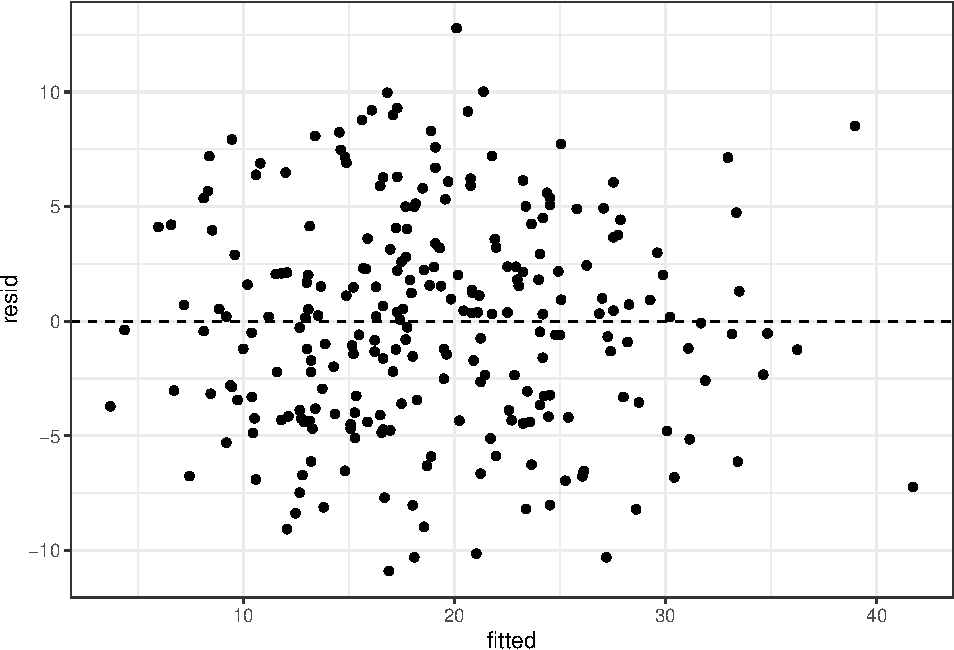
\includegraphics{CHAP23_files/figure-latex/unnamed-chunk-4-1} \end{center}

\begin{Shaded}
\begin{Highlighting}[]
\FunctionTok{ggplot}\NormalTok{(}\AttributeTok{data =}\NormalTok{ aug\_mod, }\FunctionTok{aes}\NormalTok{(}\AttributeTok{sample =}\NormalTok{ waist)) }\SpecialCharTok{+} 
  \FunctionTok{geom\_qq}\NormalTok{() }\SpecialCharTok{+}
  \FunctionTok{geom\_qq\_line}\NormalTok{() }\SpecialCharTok{+}
  \FunctionTok{theme\_bw}\NormalTok{() }
\end{Highlighting}
\end{Shaded}

\begin{center}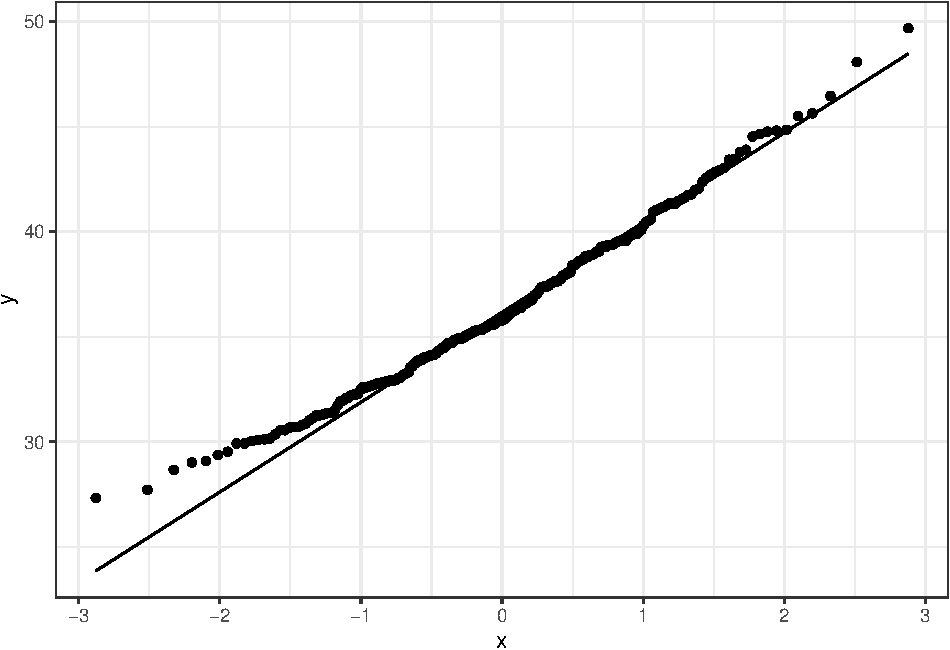
\includegraphics{CHAP23_files/figure-latex/unnamed-chunk-4-2} \end{center}

\begin{Shaded}
\begin{Highlighting}[]
\FunctionTok{library}\NormalTok{(car)}
\FunctionTok{residualPlot}\NormalTok{(mod\_lm)}
\end{Highlighting}
\end{Shaded}

\begin{center}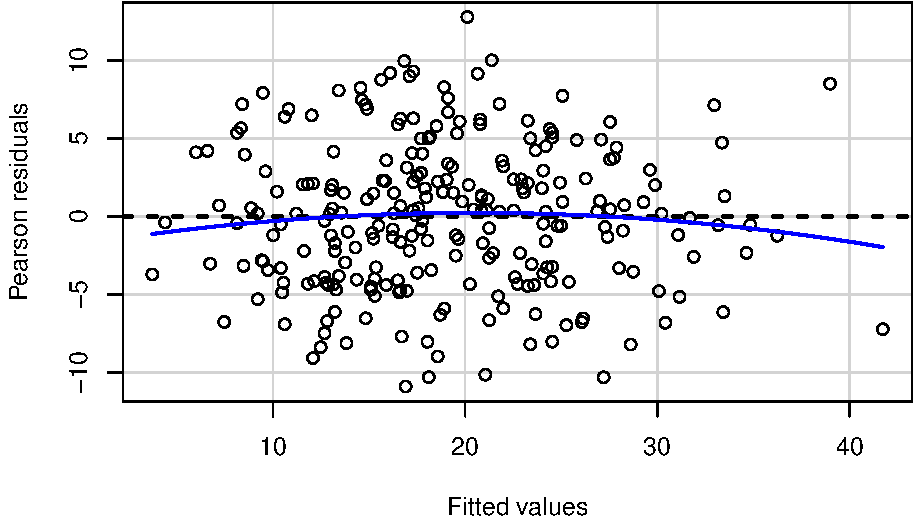
\includegraphics{CHAP23_files/figure-latex/unnamed-chunk-5-1} \end{center}

\begin{Shaded}
\begin{Highlighting}[]
\FunctionTok{qqPlot}\NormalTok{(mod\_lm)}
\end{Highlighting}
\end{Shaded}

\begin{center}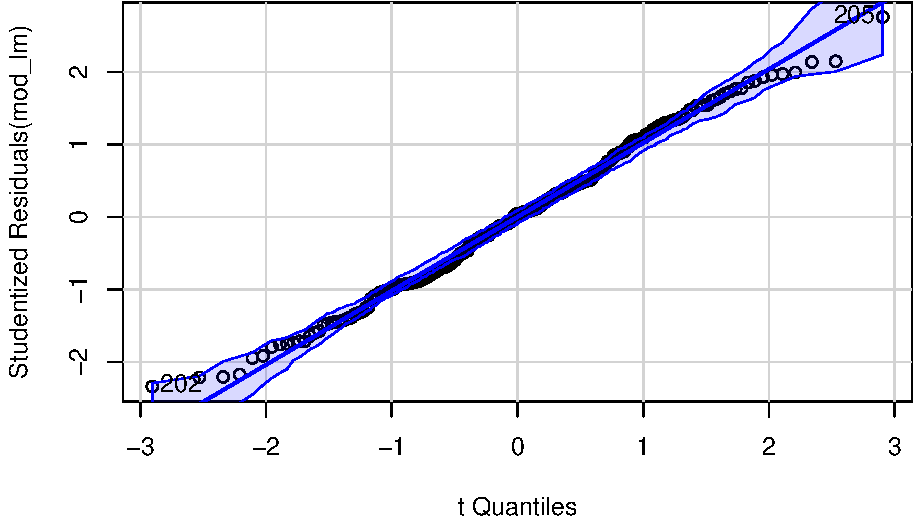
\includegraphics{CHAP23_files/figure-latex/unnamed-chunk-5-2} \end{center}

\begin{verbatim}
[1] 202 205
\end{verbatim}

\begin{Shaded}
\begin{Highlighting}[]
\CommentTok{\# Base R}
\FunctionTok{plot}\NormalTok{(mod\_lm, }\AttributeTok{which =} \DecValTok{1}\NormalTok{)}
\end{Highlighting}
\end{Shaded}

\begin{center}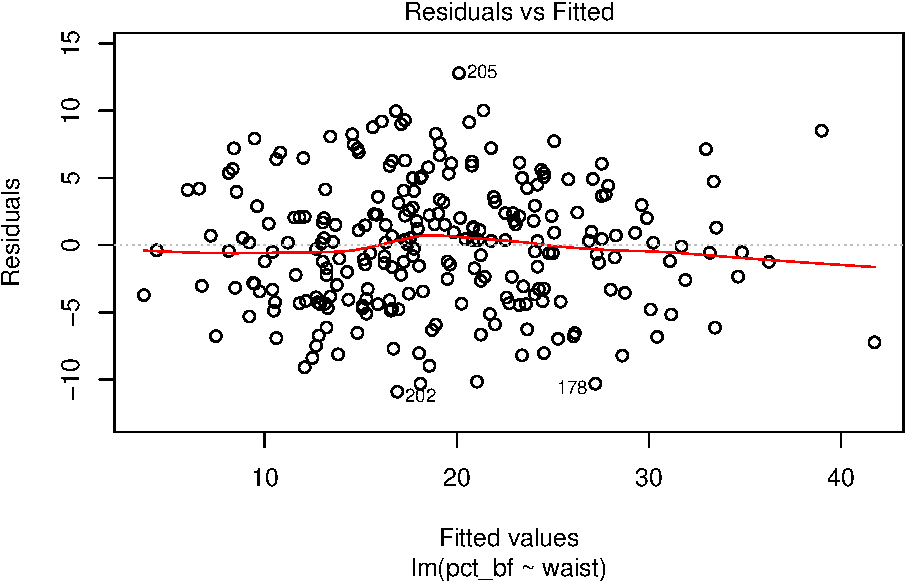
\includegraphics{CHAP23_files/figure-latex/unnamed-chunk-6-1} \end{center}

\begin{Shaded}
\begin{Highlighting}[]
\FunctionTok{plot}\NormalTok{(mod\_lm, }\AttributeTok{which =} \DecValTok{2}\NormalTok{)}
\end{Highlighting}
\end{Shaded}

\begin{center}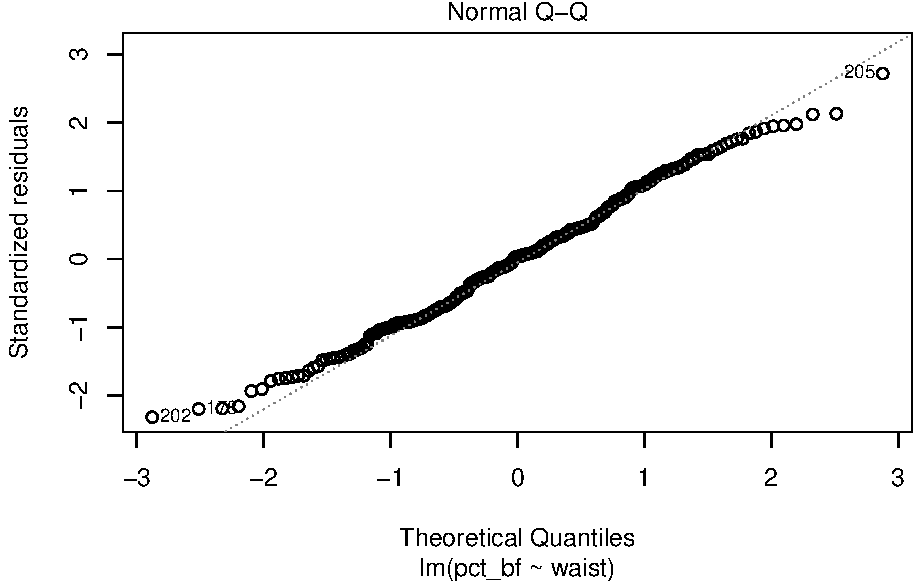
\includegraphics{CHAP23_files/figure-latex/unnamed-chunk-6-2} \end{center}

\hypertarget{residual-standard-deviation}{%
\subsection{Residual Standard Deviation}\label{residual-standard-deviation}}

\[s_{e} = \sqrt{\frac{\sum(y - \hat{y})^2}{n-2}}\]

\begin{Shaded}
\begin{Highlighting}[]
\FunctionTok{summary}\NormalTok{(mod\_lm)}
\end{Highlighting}
\end{Shaded}

\begin{verbatim}
Call:
lm(formula = pct_bf ~ waist, data = bodyfat)

Residuals:
     Min       1Q   Median       3Q      Max 
-10.8987  -3.6453   0.1864   3.1775  12.7887 

Coefficients:
             Estimate Std. Error t value Pr(>|t|)    
(Intercept) -42.73413    2.71651  -15.73   <2e-16 ***
waist         1.69997    0.07431   22.88   <2e-16 ***
---
Signif. codes:  0 '***' 0.001 '**' 0.01 '*' 0.05 '.' 0.1 ' ' 1

Residual standard error: 4.713 on 248 degrees of freedom
Multiple R-squared:  0.6785,    Adjusted R-squared:  0.6772 
F-statistic: 523.3 on 1 and 248 DF,  p-value: < 2.2e-16
\end{verbatim}

\begin{Shaded}
\begin{Highlighting}[]
\FunctionTok{summary}\NormalTok{(mod\_lm)}\SpecialCharTok{$}\NormalTok{sigma }\OtherTok{{-}\textgreater{}}\NormalTok{ s\_e}
\NormalTok{s\_e}
\end{Highlighting}
\end{Shaded}

\begin{verbatim}
[1] 4.71257
\end{verbatim}

\begin{Shaded}
\begin{Highlighting}[]
\DocumentationTok{\#\#\# By hand now}
\NormalTok{yhat }\OtherTok{\textless{}{-}} \FunctionTok{fitted}\NormalTok{(mod\_lm)}
\NormalTok{y }\OtherTok{\textless{}{-}}\NormalTok{ bodyfat}\SpecialCharTok{$}\NormalTok{pct\_bf}
\NormalTok{se1 }\OtherTok{\textless{}{-}} \FunctionTok{sqrt}\NormalTok{(}\FunctionTok{sum}\NormalTok{((y }\SpecialCharTok{{-}}\NormalTok{ yhat)}\SpecialCharTok{\^{}}\DecValTok{2}\NormalTok{)}\SpecialCharTok{/}\DecValTok{248}\NormalTok{)}
\NormalTok{se1}
\end{Highlighting}
\end{Shaded}

\begin{verbatim}
[1] 4.71257
\end{verbatim}

\hypertarget{slopes-vary-revisited}{%
\subsection{Slopes Vary Revisited}\label{slopes-vary-revisited}}

\begin{Shaded}
\begin{Highlighting}[]
\CommentTok{\# Take 1000 random samples of size 250}
\FunctionTok{set.seed}\NormalTok{(}\DecValTok{3}\NormalTok{)}
\NormalTok{n }\OtherTok{\textless{}{-}} \DecValTok{1000}
\NormalTok{b1 }\OtherTok{\textless{}{-}} \FunctionTok{numeric}\NormalTok{(n)}
\ControlFlowTok{for}\NormalTok{(i }\ControlFlowTok{in} \DecValTok{1}\SpecialCharTok{:}\NormalTok{n)\{}
\NormalTok{DF }\OtherTok{\textless{}{-}} \FunctionTok{sample\_n}\NormalTok{(bodyfat, }\AttributeTok{size =} \DecValTok{250}\NormalTok{, }\AttributeTok{replace =} \ConstantTok{TRUE}\NormalTok{)}
\NormalTok{mod }\OtherTok{\textless{}{-}} \FunctionTok{lm}\NormalTok{(pct\_bf }\SpecialCharTok{\textasciitilde{}}\NormalTok{ waist, }\AttributeTok{data =}\NormalTok{ DF)}
\NormalTok{b1[i] }\OtherTok{\textless{}{-}}\NormalTok{ mod}\SpecialCharTok{$}\NormalTok{coefficients[}\DecValTok{2}\NormalTok{]}
\NormalTok{\}}
\NormalTok{ep }\OtherTok{\textless{}{-}} \FunctionTok{quantile}\NormalTok{(b1, }\AttributeTok{probs =} \FunctionTok{c}\NormalTok{(}\FloatTok{0.025}\NormalTok{, }\FloatTok{0.975}\NormalTok{))}
\NormalTok{ep}
\end{Highlighting}
\end{Shaded}

\begin{verbatim}
    2.5%    97.5% 
1.550538 1.841983 
\end{verbatim}

\hypertarget{multiple-regression-inference}{%
\subsection{Multiple Regression Inference}\label{multiple-regression-inference}}

\begin{Shaded}
\begin{Highlighting}[]
\NormalTok{mod\_mr }\OtherTok{\textless{}{-}} \FunctionTok{lm}\NormalTok{(pct\_bf }\SpecialCharTok{\textasciitilde{}}\NormalTok{ waist }\SpecialCharTok{+}\NormalTok{ height, }\AttributeTok{data =}\NormalTok{ bodyfat)}
\FunctionTok{summary}\NormalTok{(mod\_mr)}
\end{Highlighting}
\end{Shaded}

\begin{verbatim}
Call:
lm(formula = pct_bf ~ waist + height, data = bodyfat)

Residuals:
     Min       1Q   Median       3Q      Max 
-11.1692  -3.4133  -0.0977   3.0995   9.9082 

Coefficients:
            Estimate Std. Error t value Pr(>|t|)    
(Intercept) -3.10088    7.68611  -0.403    0.687    
waist        1.77309    0.07158  24.770  < 2e-16 ***
height      -0.60154    0.10994  -5.472 1.09e-07 ***
---
Signif. codes:  0 '***' 0.001 '**' 0.01 '*' 0.05 '.' 0.1 ' ' 1

Residual standard error: 4.46 on 247 degrees of freedom
Multiple R-squared:  0.7132,    Adjusted R-squared:  0.7109 
F-statistic: 307.1 on 2 and 247 DF,  p-value: < 2.2e-16
\end{verbatim}

\hypertarget{collinearity}{%
\subsection{Collinearity}\label{collinearity}}

\begin{Shaded}
\begin{Highlighting}[]
\NormalTok{coasters }\OtherTok{\textless{}{-}} \FunctionTok{read.csv}\NormalTok{(}\StringTok{"./DATA/Coasters\_2015.csv"}\NormalTok{) }\SpecialCharTok{\%\textgreater{}\%} 
  \FunctionTok{clean\_names}\NormalTok{() }\SpecialCharTok{\%\textgreater{}\%} 
\FunctionTok{filter}\NormalTok{(name }\SpecialCharTok{!=} \StringTok{"Xcelerator"}\NormalTok{, name }\SpecialCharTok{!=} \StringTok{"Tower of Terror"}\NormalTok{)}
\NormalTok{mod\_1 }\OtherTok{\textless{}{-}} \FunctionTok{lm}\NormalTok{(duration }\SpecialCharTok{\textasciitilde{}}\NormalTok{ drop, }\AttributeTok{data =}\NormalTok{ coasters)}
\NormalTok{mod\_2 }\OtherTok{\textless{}{-}} \FunctionTok{lm}\NormalTok{(duration }\SpecialCharTok{\textasciitilde{}}\NormalTok{ drop }\SpecialCharTok{+}\NormalTok{ speed, }\AttributeTok{data =}\NormalTok{ coasters)}
\FunctionTok{summary}\NormalTok{(mod\_1)}
\end{Highlighting}
\end{Shaded}

\begin{verbatim}
Call:
lm(formula = duration ~ drop, data = coasters)

Residuals:
    Min      1Q  Median      3Q     Max 
-64.869 -18.868  -0.189  17.084  82.062 

Coefficients:
            Estimate Std. Error t value Pr(>|t|)    
(Intercept) 88.48688    9.52406   9.291 1.14e-14 ***
drop         0.38634    0.06279   6.153 2.26e-08 ***
---
Signif. codes:  0 '***' 0.001 '**' 0.01 '*' 0.05 '.' 0.1 ' ' 1

Residual standard error: 33.27 on 87 degrees of freedom
  (150 observations deleted due to missingness)
Multiple R-squared:  0.3032,    Adjusted R-squared:  0.2952 
F-statistic: 37.86 on 1 and 87 DF,  p-value: 2.264e-08
\end{verbatim}

\begin{Shaded}
\begin{Highlighting}[]
\FunctionTok{summary}\NormalTok{(mod\_2)}
\end{Highlighting}
\end{Shaded}

\begin{verbatim}
Call:
lm(formula = duration ~ drop + speed, data = coasters)

Residuals:
    Min      1Q  Median      3Q     Max 
-67.751 -16.483  -3.216  15.370  90.226 

Coefficients:
            Estimate Std. Error t value Pr(>|t|)   
(Intercept)  -6.3932    34.0567  -0.188  0.85154   
drop         -0.1399     0.1917  -0.730  0.46754   
speed         2.7030     0.9346   2.892  0.00484 **
---
Signif. codes:  0 '***' 0.001 '**' 0.01 '*' 0.05 '.' 0.1 ' ' 1

Residual standard error: 31.94 on 86 degrees of freedom
  (150 observations deleted due to missingness)
Multiple R-squared:  0.365, Adjusted R-squared:  0.3502 
F-statistic: 24.71 on 2 and 86 DF,  p-value: 3.314e-09
\end{verbatim}

\begin{Shaded}
\begin{Highlighting}[]
\CommentTok{\# from car {-}{-}{-}{-} Variance Inflation Factor vif}
\FunctionTok{vif}\NormalTok{(mod\_2)}
\end{Highlighting}
\end{Shaded}

\begin{verbatim}
   drop   speed 
10.1066 10.1066 
\end{verbatim}

\hypertarget{confidence-and-prediction-intervals}{%
\subsection{Confidence and Prediction Intervals}\label{confidence-and-prediction-intervals}}

\begin{Shaded}
\begin{Highlighting}[]
\CommentTok{\# Mean Body Fat for male with 38 inch waist {-} CI}
\FunctionTok{predict}\NormalTok{(mod\_lm, }\AttributeTok{newdata =} \FunctionTok{data.frame}\NormalTok{(}\AttributeTok{waist =} \DecValTok{38}\NormalTok{), }\AttributeTok{interval =} \StringTok{"confidence"}\NormalTok{, }\AttributeTok{level =} \FloatTok{0.95}\NormalTok{)}
\end{Highlighting}
\end{Shaded}

\begin{verbatim}
      fit     lwr      upr
1 21.8648 21.2291 22.50049
\end{verbatim}

\begin{Shaded}
\begin{Highlighting}[]
\CommentTok{\# Prediction individual with a 38 inch waist}
\FunctionTok{predict}\NormalTok{(mod\_lm, }\AttributeTok{newdata =} \FunctionTok{data.frame}\NormalTok{(}\AttributeTok{waist =} \DecValTok{38}\NormalTok{), }\AttributeTok{interval =} \StringTok{"predict"}\NormalTok{, }\AttributeTok{level =} \FloatTok{0.95}\NormalTok{)}
\end{Highlighting}
\end{Shaded}

\begin{verbatim}
      fit      lwr     upr
1 21.8648 12.56129 31.1683
\end{verbatim}

\hypertarget{logistic-regression}{%
\subsection{Logistic Regression}\label{logistic-regression}}

\begin{Shaded}
\begin{Highlighting}[]
\NormalTok{pima }\OtherTok{\textless{}{-}} \FunctionTok{read.csv}\NormalTok{(}\StringTok{"./DATA/Pima\_indians.csv"}\NormalTok{) }\SpecialCharTok{\%\textgreater{}\%} 
  \FunctionTok{clean\_names}\NormalTok{() }\SpecialCharTok{\%\textgreater{}\%} 
  \FunctionTok{filter}\NormalTok{(bmi }\SpecialCharTok{!=} \DecValTok{0}\NormalTok{)}
\FunctionTok{head}\NormalTok{(pima)}
\end{Highlighting}
\end{Shaded}

\begin{verbatim}
  diabetes  bmi age
1        1 33.6  50
2        0 26.6  31
3        1 23.3  32
4        0 28.1  21
5        1 43.1  33
6        0 25.6  30
\end{verbatim}

\begin{Shaded}
\begin{Highlighting}[]
\DocumentationTok{\#\#\#}
\FunctionTok{ggplot}\NormalTok{(}\AttributeTok{data =}\NormalTok{ pima, }\FunctionTok{aes}\NormalTok{(}\AttributeTok{x =} \FunctionTok{factor}\NormalTok{(diabetes), }\AttributeTok{y =}\NormalTok{ bmi)) }\SpecialCharTok{+} 
  \FunctionTok{geom\_boxplot}\NormalTok{() }\SpecialCharTok{+} 
  \FunctionTok{theme\_bw}\NormalTok{()}
\end{Highlighting}
\end{Shaded}

\begin{center}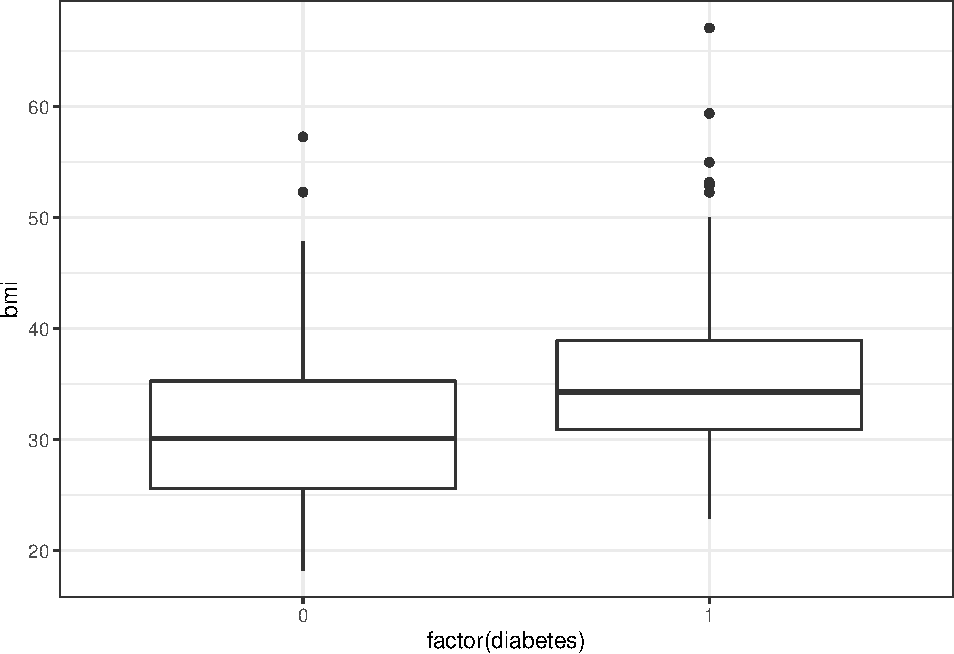
\includegraphics{CHAP23_files/figure-latex/unnamed-chunk-12-1} \end{center}

\begin{Shaded}
\begin{Highlighting}[]
\DocumentationTok{\#\#\#}
\FunctionTok{ggplot}\NormalTok{(}\AttributeTok{data =}\NormalTok{ pima, }\FunctionTok{aes}\NormalTok{(}\AttributeTok{x =}\NormalTok{ bmi, }\AttributeTok{y =}\NormalTok{ diabetes)) }\SpecialCharTok{+} 
  \FunctionTok{geom\_point}\NormalTok{() }\SpecialCharTok{+}
  \FunctionTok{theme\_bw}\NormalTok{() }\SpecialCharTok{+} 
  \FunctionTok{geom\_smooth}\NormalTok{(}\AttributeTok{method =} \StringTok{"glm"}\NormalTok{, }\AttributeTok{method.args =} \FunctionTok{list}\NormalTok{(}\AttributeTok{family =} \StringTok{"binomial"}\NormalTok{))}
\end{Highlighting}
\end{Shaded}

\begin{center}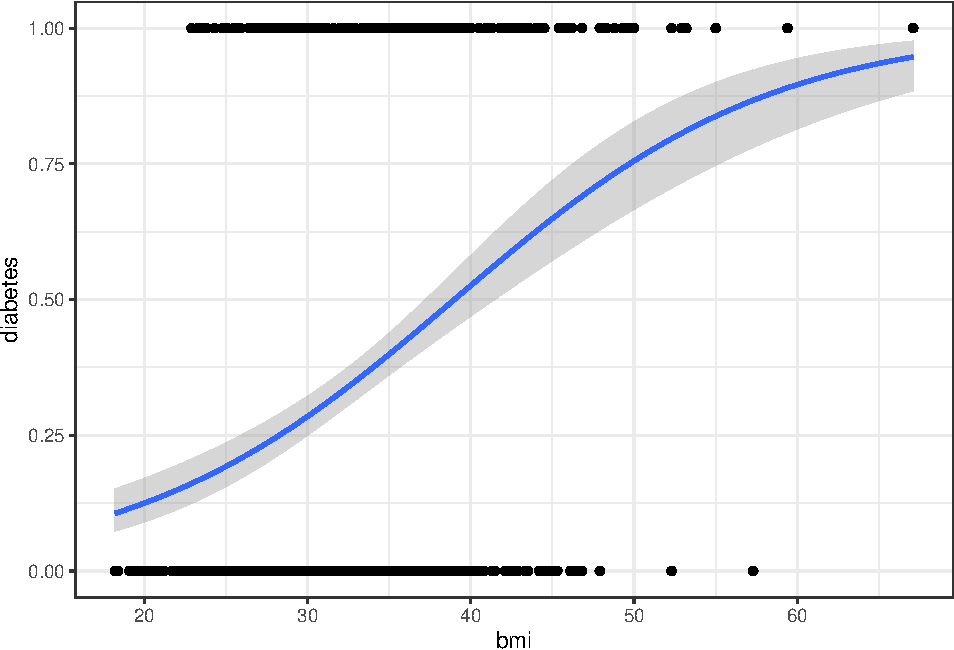
\includegraphics{CHAP23_files/figure-latex/unnamed-chunk-12-2} \end{center}

\begin{Shaded}
\begin{Highlighting}[]
\NormalTok{mod\_lr }\OtherTok{\textless{}{-}} \FunctionTok{glm}\NormalTok{(diabetes }\SpecialCharTok{\textasciitilde{}}\NormalTok{ bmi, }\AttributeTok{data =}\NormalTok{ pima, }\AttributeTok{family =} \StringTok{"binomial"}\NormalTok{)}
\FunctionTok{summary}\NormalTok{(mod\_lr)}
\end{Highlighting}
\end{Shaded}

\begin{verbatim}
Call:
glm(formula = diabetes ~ bmi, family = "binomial", data = pima)

Deviance Residuals: 
    Min       1Q   Median       3Q      Max  
-2.0094  -0.9184  -0.6598   1.2254   1.9107  

Coefficients:
            Estimate Std. Error z value Pr(>|z|)    
(Intercept) -3.99682    0.42885   -9.32  < 2e-16 ***
bmi          0.10250    0.01261    8.13 4.31e-16 ***
---
Signif. codes:  0 '***' 0.001 '**' 0.01 '*' 0.05 '.' 0.1 ' ' 1

(Dispersion parameter for binomial family taken to be 1)

    Null deviance: 981.53  on 756  degrees of freedom
Residual deviance: 904.89  on 755  degrees of freedom
AIC: 908.89

Number of Fisher Scoring iterations: 4
\end{verbatim}

\begin{Shaded}
\begin{Highlighting}[]
\FunctionTok{predict}\NormalTok{(mod\_lr, }\AttributeTok{newdata =} \FunctionTok{data.frame}\NormalTok{(}\AttributeTok{bmi =} \DecValTok{60}\NormalTok{), }\AttributeTok{type =} \StringTok{"response"}\NormalTok{)}
\end{Highlighting}
\end{Shaded}

\begin{verbatim}
        1 
0.8959635 
\end{verbatim}

\hypertarget{problems}{%
\subsection{Problems}\label{problems}}

\begin{Shaded}
\begin{Highlighting}[]
\NormalTok{earnings }\OtherTok{\textless{}{-}} \FunctionTok{read.csv}\NormalTok{(}\StringTok{"./DATA/Graduate\_Earnings.csv"}\NormalTok{) }\SpecialCharTok{\%\textgreater{}\%} 
  \FunctionTok{clean\_names}\NormalTok{()}
\FunctionTok{head}\NormalTok{(earnings)}
\end{Highlighting}
\end{Shaded}

\begin{verbatim}
                             school public      location  earn  sat act price
1              Princeton University      0 Princeton, NJ 62800 1510  33 61300
2  University of Michigan-Ann Arbor      1 Ann Arbor, MI 59000 1380  30 28100
3                Harvard University      0 Cambridge, MA 62900 1510  34 64800
4                   Rice University      0   Houston, TX 63700 1460  33 58600
5 University of California-Berkeley      1  Berkeley, CA 60300 1360  30 35700
6    Brigham Young University-Provo      1     Provo, UT 51800 1260  29 18500
  price_with_aid need_fraction merit_aided
1          20600          0.59          NA
2          17300          0.30        0.16
3          16500          0.58          NA
4          22400          0.39        0.11
5          18200          0.51        0.06
6          13400          0.39        0.24
\end{verbatim}

\begin{Shaded}
\begin{Highlighting}[]
\NormalTok{mod }\OtherTok{\textless{}{-}} \FunctionTok{lm}\NormalTok{(earn }\SpecialCharTok{\textasciitilde{}}\NormalTok{ sat, }\AttributeTok{data =}\NormalTok{ earnings)}
\FunctionTok{summary}\NormalTok{(mod)}
\end{Highlighting}
\end{Shaded}

\begin{verbatim}
Call:
lm(formula = earn ~ sat, data = earnings)

Residuals:
     Min       1Q   Median       3Q      Max 
-16385.1  -3521.6   -246.4   3191.6  24881.0 

Coefficients:
             Estimate Std. Error t value Pr(>|t|)    
(Intercept) 14468.088   1776.682   8.143 1.75e-15 ***
sat            27.264      1.545  17.646  < 2e-16 ***
---
Signif. codes:  0 '***' 0.001 '**' 0.01 '*' 0.05 '.' 0.1 ' ' 1

Residual standard error: 5603 on 704 degrees of freedom
Multiple R-squared:  0.3067,    Adjusted R-squared:  0.3057 
F-statistic: 311.4 on 1 and 704 DF,  p-value: < 2.2e-16
\end{verbatim}

\begin{Shaded}
\begin{Highlighting}[]
\FunctionTok{confint}\NormalTok{(mod)}
\end{Highlighting}
\end{Shaded}

\begin{verbatim}
                  2.5 %      97.5 %
(Intercept) 10979.85867 17956.31734
sat            24.23067    30.29765
\end{verbatim}

\begin{Shaded}
\begin{Highlighting}[]
\NormalTok{mod2 }\OtherTok{\textless{}{-}} \FunctionTok{lm}\NormalTok{(earn }\SpecialCharTok{\textasciitilde{}}\NormalTok{ sat }\SpecialCharTok{+}\NormalTok{ need\_fraction, }\AttributeTok{data =}\NormalTok{ earnings)}
\FunctionTok{summary}\NormalTok{(mod2)}
\end{Highlighting}
\end{Shaded}

\begin{verbatim}
Call:
lm(formula = earn ~ sat + need_fraction, data = earnings)

Residuals:
   Min     1Q Median     3Q    Max 
-16409  -3819   -423   2832  25658 

Coefficients:
               Estimate Std. Error t value Pr(>|t|)    
(Intercept)   23974.208   2327.479  10.301  < 2e-16 ***
sat              23.188      1.658  13.989  < 2e-16 ***
need_fraction -8500.746   1328.938  -6.397 2.94e-10 ***
---
Signif. codes:  0 '***' 0.001 '**' 0.01 '*' 0.05 '.' 0.1 ' ' 1

Residual standard error: 5409 on 684 degrees of freedom
  (19 observations deleted due to missingness)
Multiple R-squared:  0.3555,    Adjusted R-squared:  0.3536 
F-statistic: 188.6 on 2 and 684 DF,  p-value: < 2.2e-16
\end{verbatim}

\begin{Shaded}
\begin{Highlighting}[]
\NormalTok{mod3 }\OtherTok{\textless{}{-}} \FunctionTok{lm}\NormalTok{(earn }\SpecialCharTok{\textasciitilde{}}\NormalTok{ sat }\SpecialCharTok{+}\NormalTok{ need\_fraction }\SpecialCharTok{+}\NormalTok{ act, }\AttributeTok{data =}\NormalTok{ earnings)}
\FunctionTok{summary}\NormalTok{(mod3)}
\end{Highlighting}
\end{Shaded}

\begin{verbatim}
Call:
lm(formula = earn ~ sat + need_fraction + act, data = earnings)

Residuals:
     Min       1Q   Median       3Q      Max 
-15653.3  -3633.6   -443.2   2822.6  25111.7 

Coefficients:
               Estimate Std. Error t value Pr(>|t|)    
(Intercept)   25162.762   2340.317  10.752  < 2e-16 ***
sat              10.112      4.355   2.322  0.02053 *  
need_fraction -8564.027   1319.930  -6.488 1.67e-10 ***
act             551.243    169.957   3.243  0.00124 ** 
---
Signif. codes:  0 '***' 0.001 '**' 0.01 '*' 0.05 '.' 0.1 ' ' 1

Residual standard error: 5372 on 683 degrees of freedom
  (19 observations deleted due to missingness)
Multiple R-squared:  0.3653,    Adjusted R-squared:  0.3625 
F-statistic:   131 on 3 and 683 DF,  p-value: < 2.2e-16
\end{verbatim}

\begin{Shaded}
\begin{Highlighting}[]
\FunctionTok{predict}\NormalTok{(mod3, }\AttributeTok{newdata =} \FunctionTok{data.frame}\NormalTok{(}\AttributeTok{sat =} \DecValTok{1200}\NormalTok{, }\AttributeTok{need\_fraction =} \FloatTok{0.5}\NormalTok{, }\AttributeTok{act =} \DecValTok{26}\NormalTok{), }\AttributeTok{interval =} \StringTok{"confidence"}\NormalTok{)}
\end{Highlighting}
\end{Shaded}

\begin{verbatim}
       fit      lwr      upr
1 47347.06 46881.35 47812.78
\end{verbatim}

\begin{Shaded}
\begin{Highlighting}[]
\FunctionTok{predict}\NormalTok{(mod3, }\AttributeTok{newdata =} \FunctionTok{data.frame}\NormalTok{(}\AttributeTok{sat =} \DecValTok{1200}\NormalTok{, }\AttributeTok{need\_fraction =} \FloatTok{0.5}\NormalTok{, }\AttributeTok{act =} \DecValTok{26}\NormalTok{), }\AttributeTok{interval =} \StringTok{"predict"}\NormalTok{)}
\end{Highlighting}
\end{Shaded}

\begin{verbatim}
       fit     lwr      upr
1 47347.06 36789.2 57904.93
\end{verbatim}

\end{document}
